\chapter{Ordering of nodes, edges, surfaces and elements}

%%%%%%%%%%%%%%%%%%%%%%%%%%%%%%%%%%%%%%%%%%%%%%%%%%%%
%%%%%%%%%%%%%%%%%%%%%%%%%%%%%%%%%%%%%%%%%%%%%%%%%%%%
\section{Plane elements}

%%%%%%%%%%%%%%%%%%%%%%%%%%%%%%%%%%%%%%%%%%%%%%%%%%%%
%%%%%%%%%%%%%%%%%%%%%%%%%%%%%%%%%%%%%%%%%%%%%%%%%%%%
\subsection{Triangular elements}

%%%%%%%%%%%%%%%%%%%%%%%%%%%%%%%%%%%%%%%%%%%%%%%%%%%%
\subsubsection{Triangular elements with three nodes}

\begin{table}[h]
\begin{center}
\begin{tabular}{|l|l|}
\hline
edge number & node numbers
\\ \hline
1 & 1, 2
\\ \hline
2 & 2, 3
\\ \hline
3 & 3, 1
\\ \hline
\end{tabular}
\label{tablintriangedges}
\caption{Ordering of edges for triangular element with 3 nodes.}
\end{center}
\end{table}

\begin{figure}[h]
\begin{center}
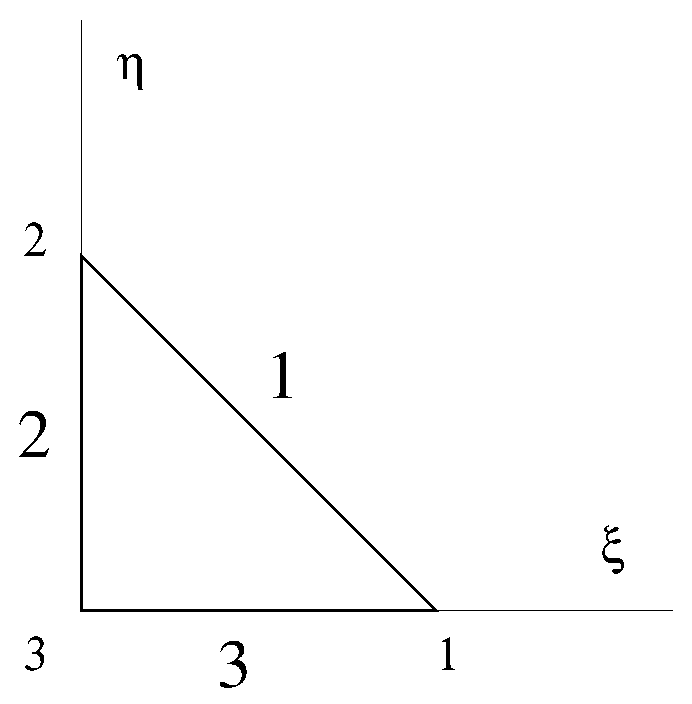
\includegraphics[width=60mm]{FIG/lintriangedges.eps}
\label{figlintriangedges}
\caption{Ordering of edges for triangular element with 3 nodes.}
\end{center}
\end{figure}

%%%%%%%%%%%%%%%%%%%%%%%%%%%%%%%%%%%%%%%%%%%%%%%%%%%%
\subsubsection{Triangular elements with six nodes}

\begin{table}[h]
\begin{center}
\begin{tabular}{|l|l|}
\hline
edge number & node numbers
\\ \hline
1 & 1, 2, 4
\\ \hline
2 & 2, 3, 5
\\ \hline
3 & 3, 1, 6
\\ \hline
\end{tabular}
\label{tabquadtriangedges}
\caption{Ordering of edges for triangular element with 6 nodes.}
\end{center}
\end{table}

\begin{figure}[h]
\begin{center}
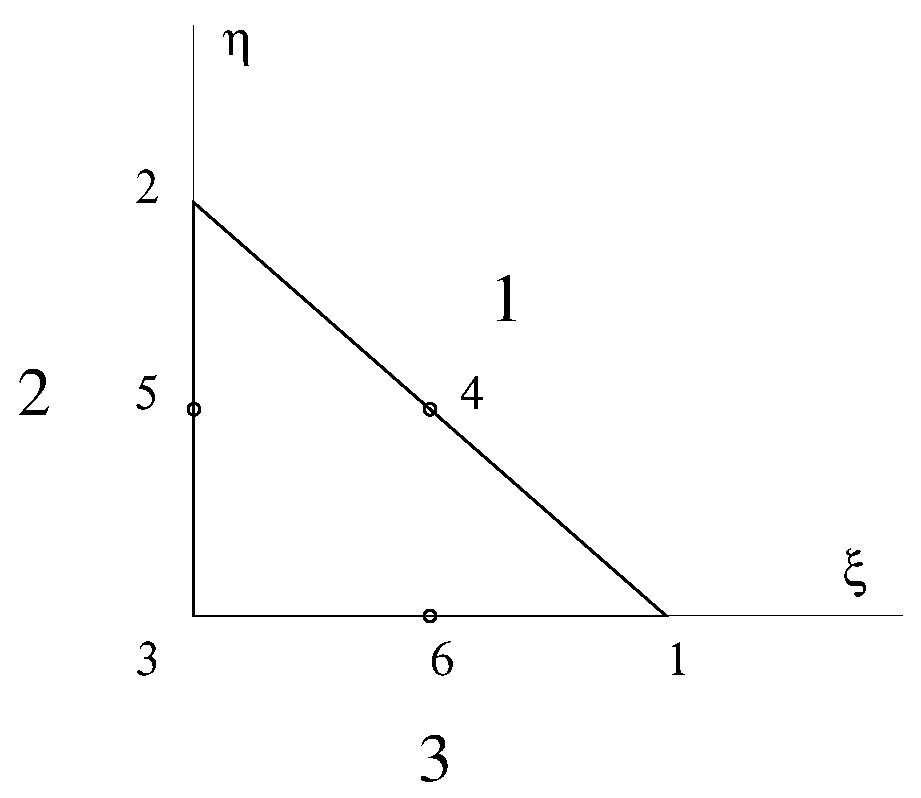
\includegraphics[width=80mm]{FIG/quadtriangedges.eps}
\label{figquadtriangedges}
\caption{Ordering of edges for triangular element with 6 nodes.}
\end{center}
\end{figure}

%%%%%%%%%%%%%%%%%%%%%%%%%%%%%%%%%%%%%%%%%%%%%
%%%%%%%%%%%%%%%%%%%%%%%%%%%%%%%%%%%%%%%%%%%%%
\subsection{Quadrilateral elements}

%%%%%%%%%%%%%%%%%%%%%%%%%%%%%%%%%%%%%%%%%%%%%
\subsubsection{Quadrilateral elements with four nodes}

\begin{table}[h]
\begin{center}
\begin{tabular}{|l|l|}
\hline
edge number & node numbers
\\ \hline
1 & 1, 2
\\ \hline
2 & 2, 3
\\ \hline
3 & 3, 4
\\ \hline
4 & 4, 1
\\ \hline
\end{tabular}
\label{tablinquadedges}
\caption{Ordering of edges for quadrilateral element with 4 nodes.}
\end{center}
\end{table}

\begin{figure}[h]
\begin{center}
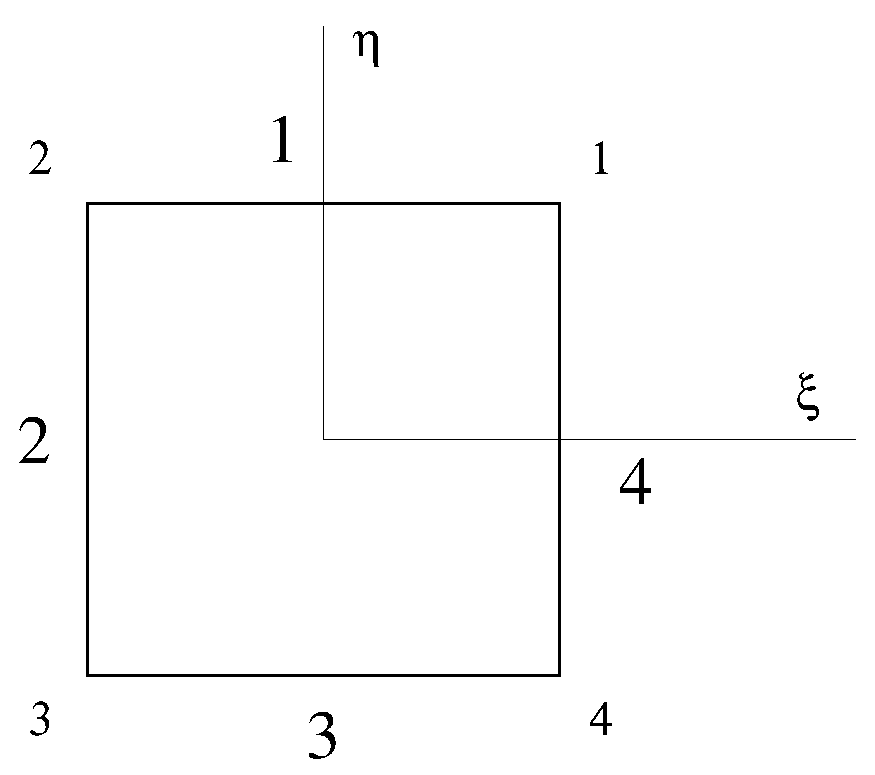
\includegraphics[width=60mm]{FIG/linquadedges.eps}
\label{figlinquadedges}
\caption{Ordering of edges for quadrilateral element with 4 nodes.}
\end{center}
\end{figure}

%%%%%%%%%%%%%%%%%%%%%%%%%%%%%%%%%%%%%%%%%%%%%
\subsubsection{Quadrilateral elements with eight nodes}

\begin{table}[h]
\begin{center}
\begin{tabular}{|l|l|}
\hline
edge number & node numbers
\\ \hline
1 & 1, 2, 5
\\ \hline
2 & 2, 3, 6
\\ \hline
3 & 3, 4, 7
\\ \hline
4 & 4, 1, 8
\\ \hline
\end{tabular}
\label{tabquadquadedges}
\caption{Ordering of edges for quadrilateral element with 8 nodes.}
\end{center}
\end{table}

\begin{figure}[h]
\begin{center}
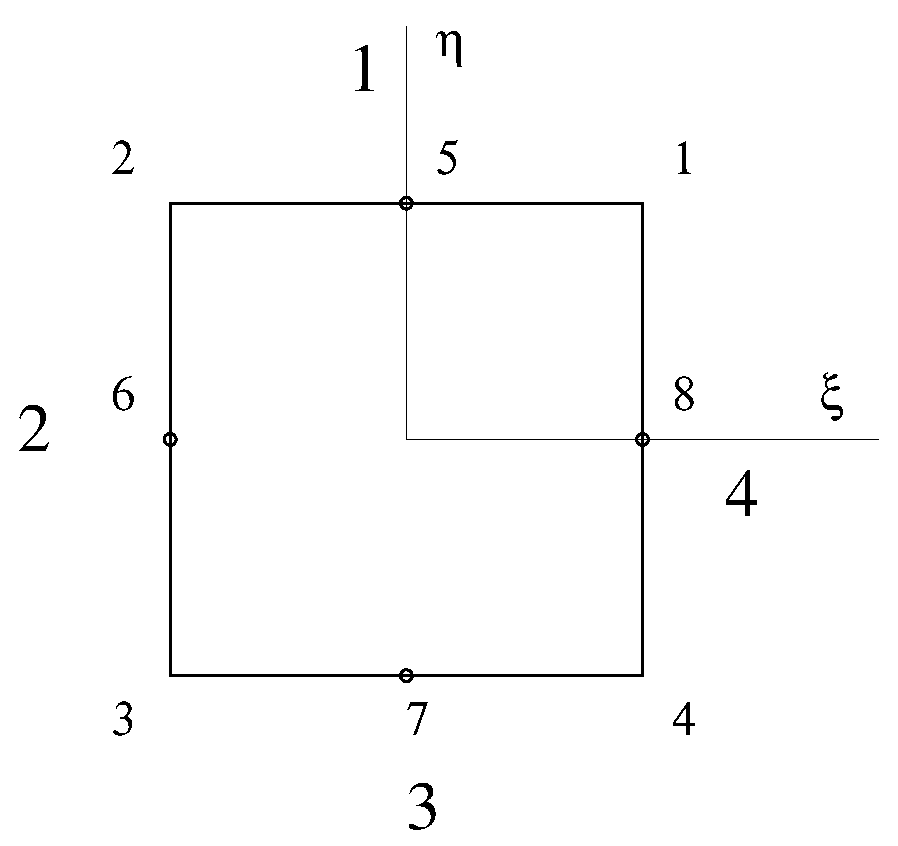
\includegraphics[width=60mm]{FIG/quadquadedges.eps}
\label{figquadquadedges}
\caption{Ordering of edges for quadrilateral element with 8 nodes.}
\end{center}
\end{figure}

%%%%%%%%%%%%%%%%%%%%%%%%%%%%%%%%%%%%%%%%%%%%%
%%%%%%%%%%%%%%%%%%%%%%%%%%%%%%%%%%%%%%%%%%%%%
\subsection{Hexahedral elements}

%%%%%%%%%%%%%%%%%%%%%%%%%%%%%%%%%%%%%%%%%%%%%
\subsubsection{Hexahedral elements with eight nodes}

\begin{table}[h]
\begin{center}
\begin{tabular}{|l|l|}
\hline
surface number & node numbers
\\ \hline
1 & 1, 4, 8, 5
\\ \hline
2 & 2, 1, 5, 6
\\ \hline
3 & 3, 2, 6, 7
\\ \hline
4 & 4, 3, 7, 8
\\ \hline
5 & 1, 2, 3, 4
\\ \hline
6 & 5, 6, 7, 8
\\ \hline
\end{tabular}
\label{tablinhexsurf}
\caption{Ordering of surfaces for hexahedral element with 8 nodes.}
\end{center}
\end{table}

\begin{figure}[h]
\begin{center}
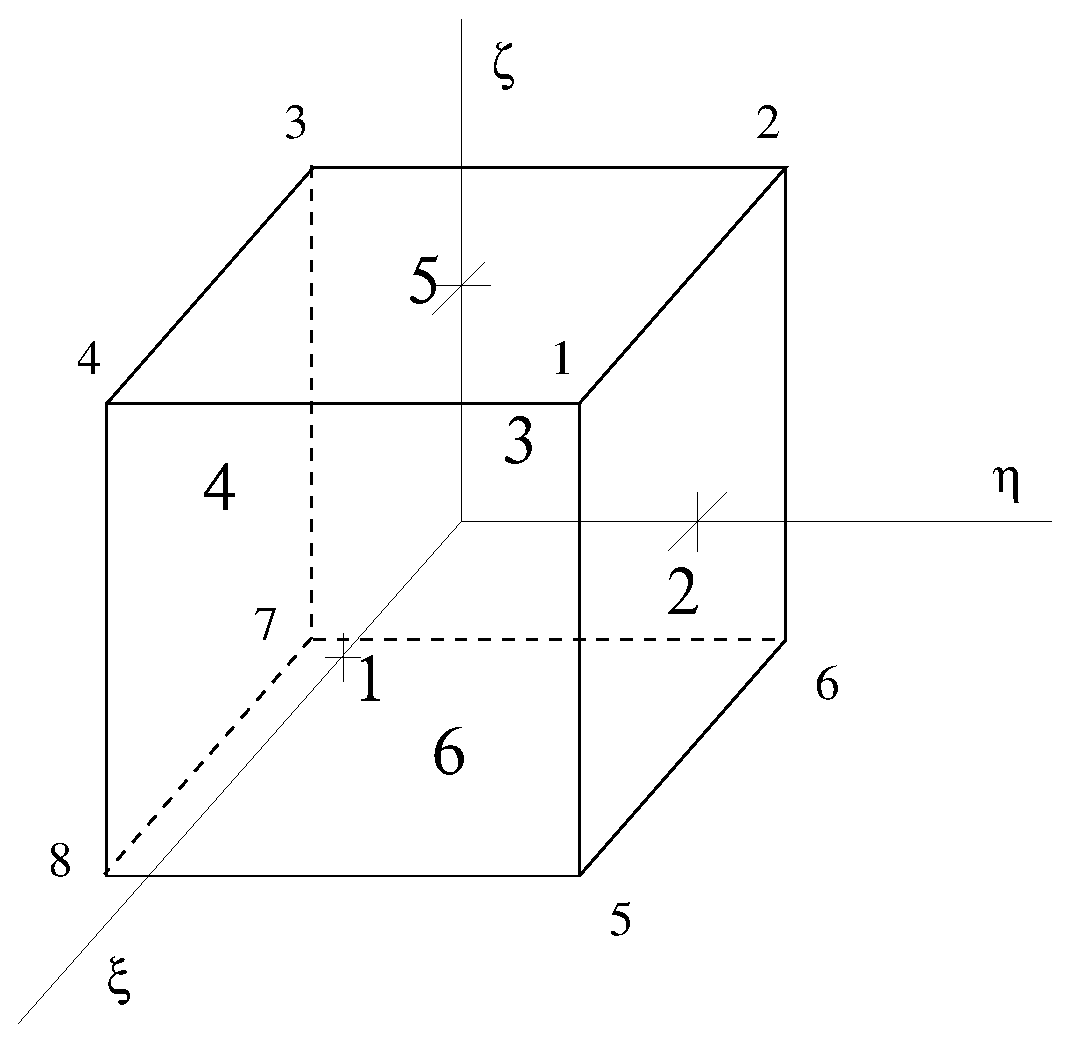
\includegraphics[width=60mm]{FIG/linhexsurf.eps}
\label{figlinhexsurf}
\caption{Ordering of surfaces for hexahedral element with 8 nodes.}
\end{center}
\end{figure}

%%%%%%%%%%%%%%%%%%%%%%%%%%%%%%%%%%%%%%%%%%%%%
\subsubsection{Hexahedral elements with twenty nodes}

\begin{table}[h]
\begin{center}
\begin{tabular}{|l|l|}
\hline
surface number & node numbers
\\ \hline
1 & 1, 4, 8, 5, 12, 16, 20, 13
\\ \hline
2 & 2, 1, 5, 6, 9, 13, 17, 14
\\ \hline
3 & 3, 2, 6, 7, 10, 14, 18, 15
\\ \hline
4 & 4, 3, 7, 8, 11, 15, 19, 16
\\ \hline
5 & 1, 2, 3, 4, 9, 10, 11, 12
\\ \hline
6 & 5, 6, 7, 8, 17, 18, 19, 20
\\ \hline
\end{tabular}
\label{tabquadhexsurf}
\caption{Ordering of surfaces for hexahedral element with 20 nodes.}
\end{center}
\end{table}

\begin{figure}[h]
\begin{center}
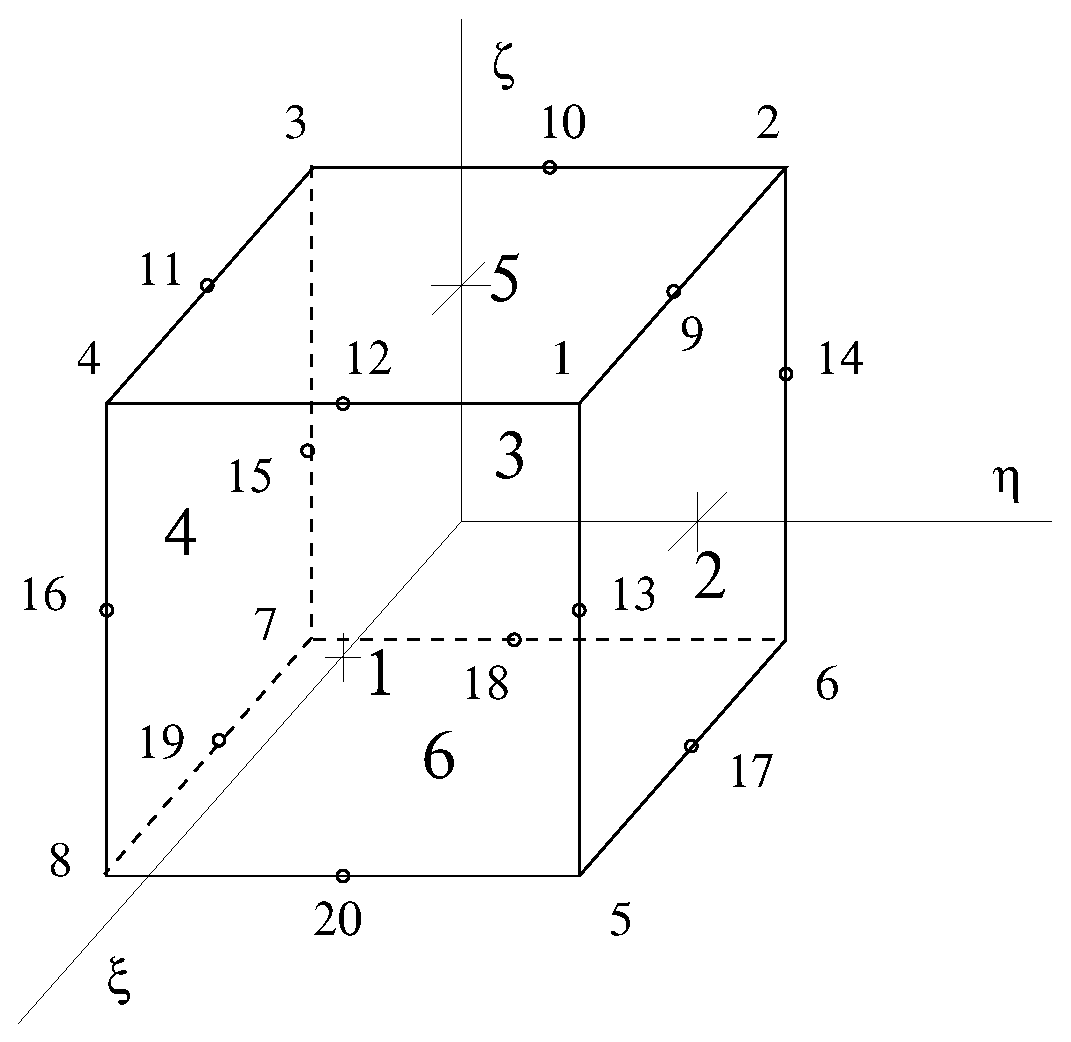
\includegraphics[width=60mm]{FIG/quadhexsurf.eps}
\label{figquadhexsurf}
\caption{Ordering of surfaces for hexahedral element with 20 nodes.}
\end{center}
\end{figure}
